\chapter{Integrity}


This chapter will present the other aspect of cryptography : tampering prevention. An adversary can be able to do more than just eavesdropping : he can actually modify ciphertext messages on-the-go (using fro example a Man in the Middle attack). Therefore we need methods to ensure the non modification of the message during transmission.\\
In Dan Boneh's lecture, the integrity enforcement mechanisms are a minor part of the course, so this chapter will be quite succinct (especially since some generic constructions were already explained in the confidentiality chapter).


\section{Message Authentication Code (MAC)}

The most common way to enforce message integrity is to add a tag to the message, which will be verified upon reception. Moreover, the tag needs to be created using a secret key in order to prevent an attacker from fooling the verification algorithm.

\begin{mydef} $MAC = (S,V)$  
\begin{flushright}
	\begin{minipage}[t]{0.45\textwidth}
		\indent   	Tag Generator \\
		\indent      $S: (k,m) -> t$   \\
	\end{minipage}
	\begin{minipage}[t]{0.45\textwidth}
		\indent	Verification Algorithm \\
		\indent    $V: (k,m,t) -> {0,1}$ \\
	\end{minipage}
\end{flushright}
\end{mydef}

The tag and tag generation are more often called respectively ``hash'' and ``hashing''  : a hash function is an algorithm which takes variable-length data as input and outputs a fixed-length image of the input data. While being created in order to lessen the memory footprint of databases and speed-up the lookup of elements (hash tables, caches), hashing functions are also vastly used in cryptography. 
 
\subsection{Secure Mac}

The experiment needed to describe the security of a MAC mechanism is the same as for the cipher's semantic security : the attacker can submit 2 messages q times, and receive the tag of n ones. If it can't forge a new valid pair (m,t) to submit to V with a significant advantage, the MAC algorithm is considered secure.

\subsection{Collision Resistance}

The strength of a MAC against forged tags are closely related to the algorithm's resistance against collision attacks. A collision is a pair of messages $(m_0,m_1)$ such that $H(m_0) == H(m_1)$. We can clearly see that $m_0$ and $m_1$, if the MAC is using the hash functions $H$, have great chances to have the same tag. The verification algorithm will take one for another, which is a breach of security. \\
Therefore the algorithm for the tag generator has to be built upon collision resistant hashing functions.


\subsection{MAC Padding}
\label{sec:ISOPadding}

As for block ciphers, a hash algorithm works usually on a fixed length of plaintext information. However, contrary to the former, it is not possible to just pad the input text with 0's because it is insecure : the attacker can then send parts of the same message to retrieve important parts of information (block length, last digit digest ). \\
The standard (ISO) currently used is to pad with one $1$ and the rest with $0$'s.


\section{Constructions}

\subsection{Construction from PRF}

A secure MAC can be easily constructed from a PRF family. The following theorem is important since a lot of real-world MAC use it, in various environment (Internet, Banks, Defence, ..). 

\begin{mytheorem}
    If $F:K\times X \leftarrow Y$ is a secure PRF and $card(Y)$ is large, then $I_F = (F, V_F)$ is a secure MAC and : 
   	\begin{flushright}
	    $ Adv_{MAC} \leq Adv_{PRF} + \frac{1}{|Y|} $
	\end{flushright}
\end{mytheorem}

The main interest of this theorem is we can produce fairly large hash function from concise pseudorandom function, as long as the output domain is large. The following paragraph will present well-known constructions to treat large input files.

\paragraph{CBC-MAC}

\begin{figure}[h!]
	\centering
		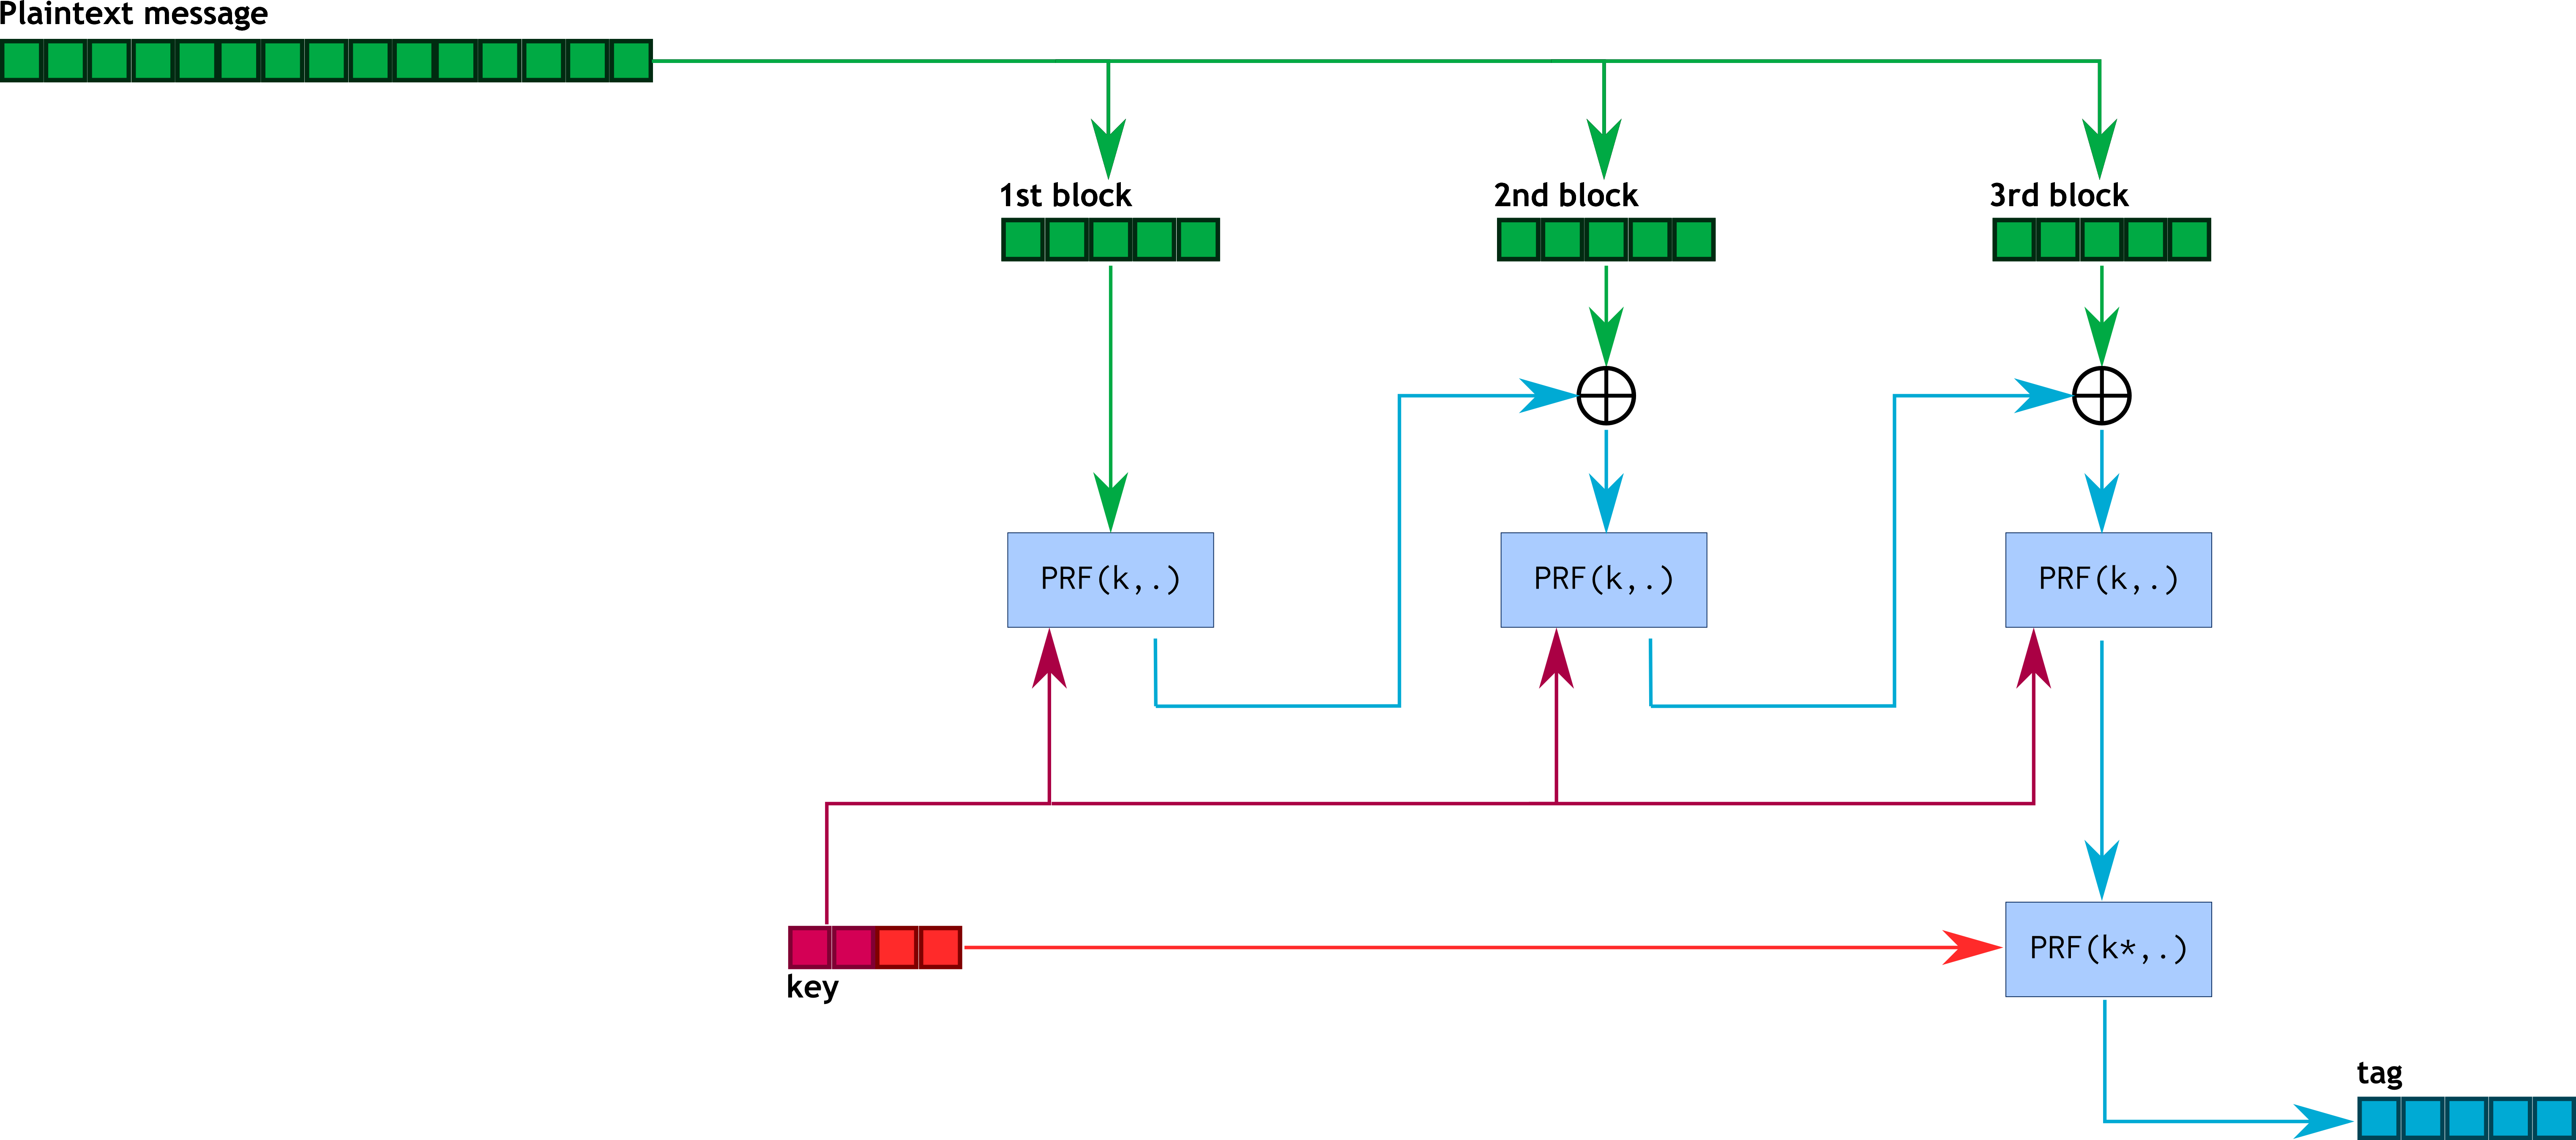
\includegraphics[width=0.7\textwidth]{CBC-MAC.PNG}
	\caption{CBC-MAC construction}
	\label{fig:CBCMACConstruction}
\end{figure}

The CBC-MAC is constructed from a single PRP by cascading the output of the previous block into the current block's input. The last tag is pad with ??? and then hashed a final time with a different key. Finally, the last block is hashed by the same function but with a different key to produce the tag.

\begin{mytheorem}
	For every q-query adversary A attacking the CBC-MAC, there exist an adversary B attacking the PRP function F such that : 
	\begin{flushright}
 		$Adv_{PRP}[A,F_{ECBC}] = Adv_{PRP}[B, F] + 2\times \frac{q^2}{2.|K|}$	
	\end{flushright}
\end{mytheorem}



\paragraph{NMAC}


\begin{figure}[h!]
	\centering
		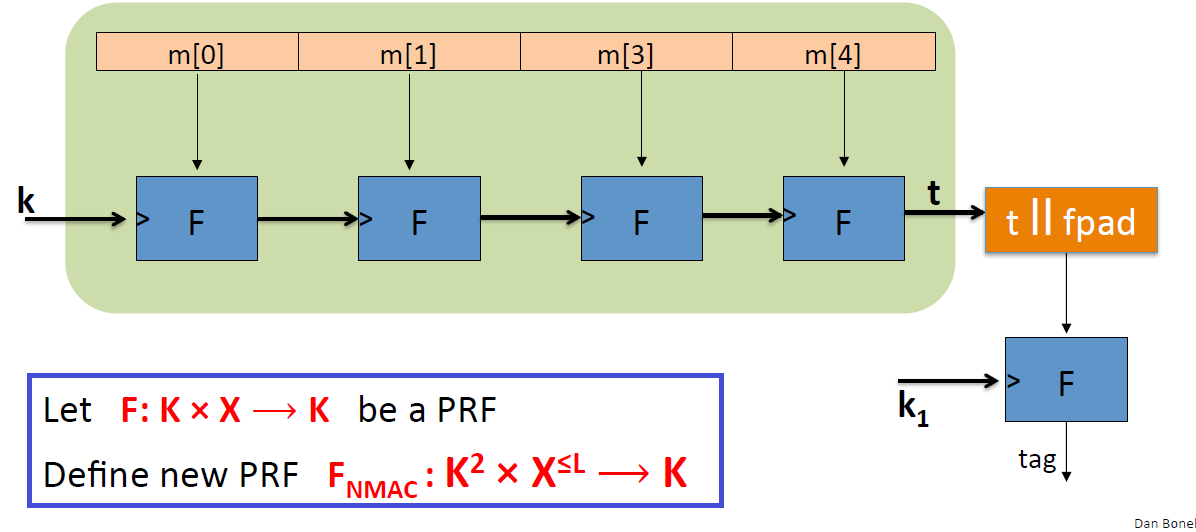
\includegraphics[width=0.7\textwidth]{NMAC.PNG}
	\caption{NMAC construction}
	\label{fig:NMACConstruction}
\end{figure}

In the NMAC construction, the output of a a block is used as the key for the next block. Like CBC-MAC, the process is fundamentally sequential.


\begin{mytheorem}
	For every q-query adversary A attacking the NMAC, there exist an adversary B attacking the PRF function F such that : 
	\begin{flushright}
 		$Adv_{PRF}[A,F_{NMAC}] = Adv_{PRF}[B, F] + 2\times \frac{q^2}{|X|}$	
	\end{flushright}
\end{mytheorem}



\paragraph{PMAC}

\begin{figure}[h!]
	\centering
		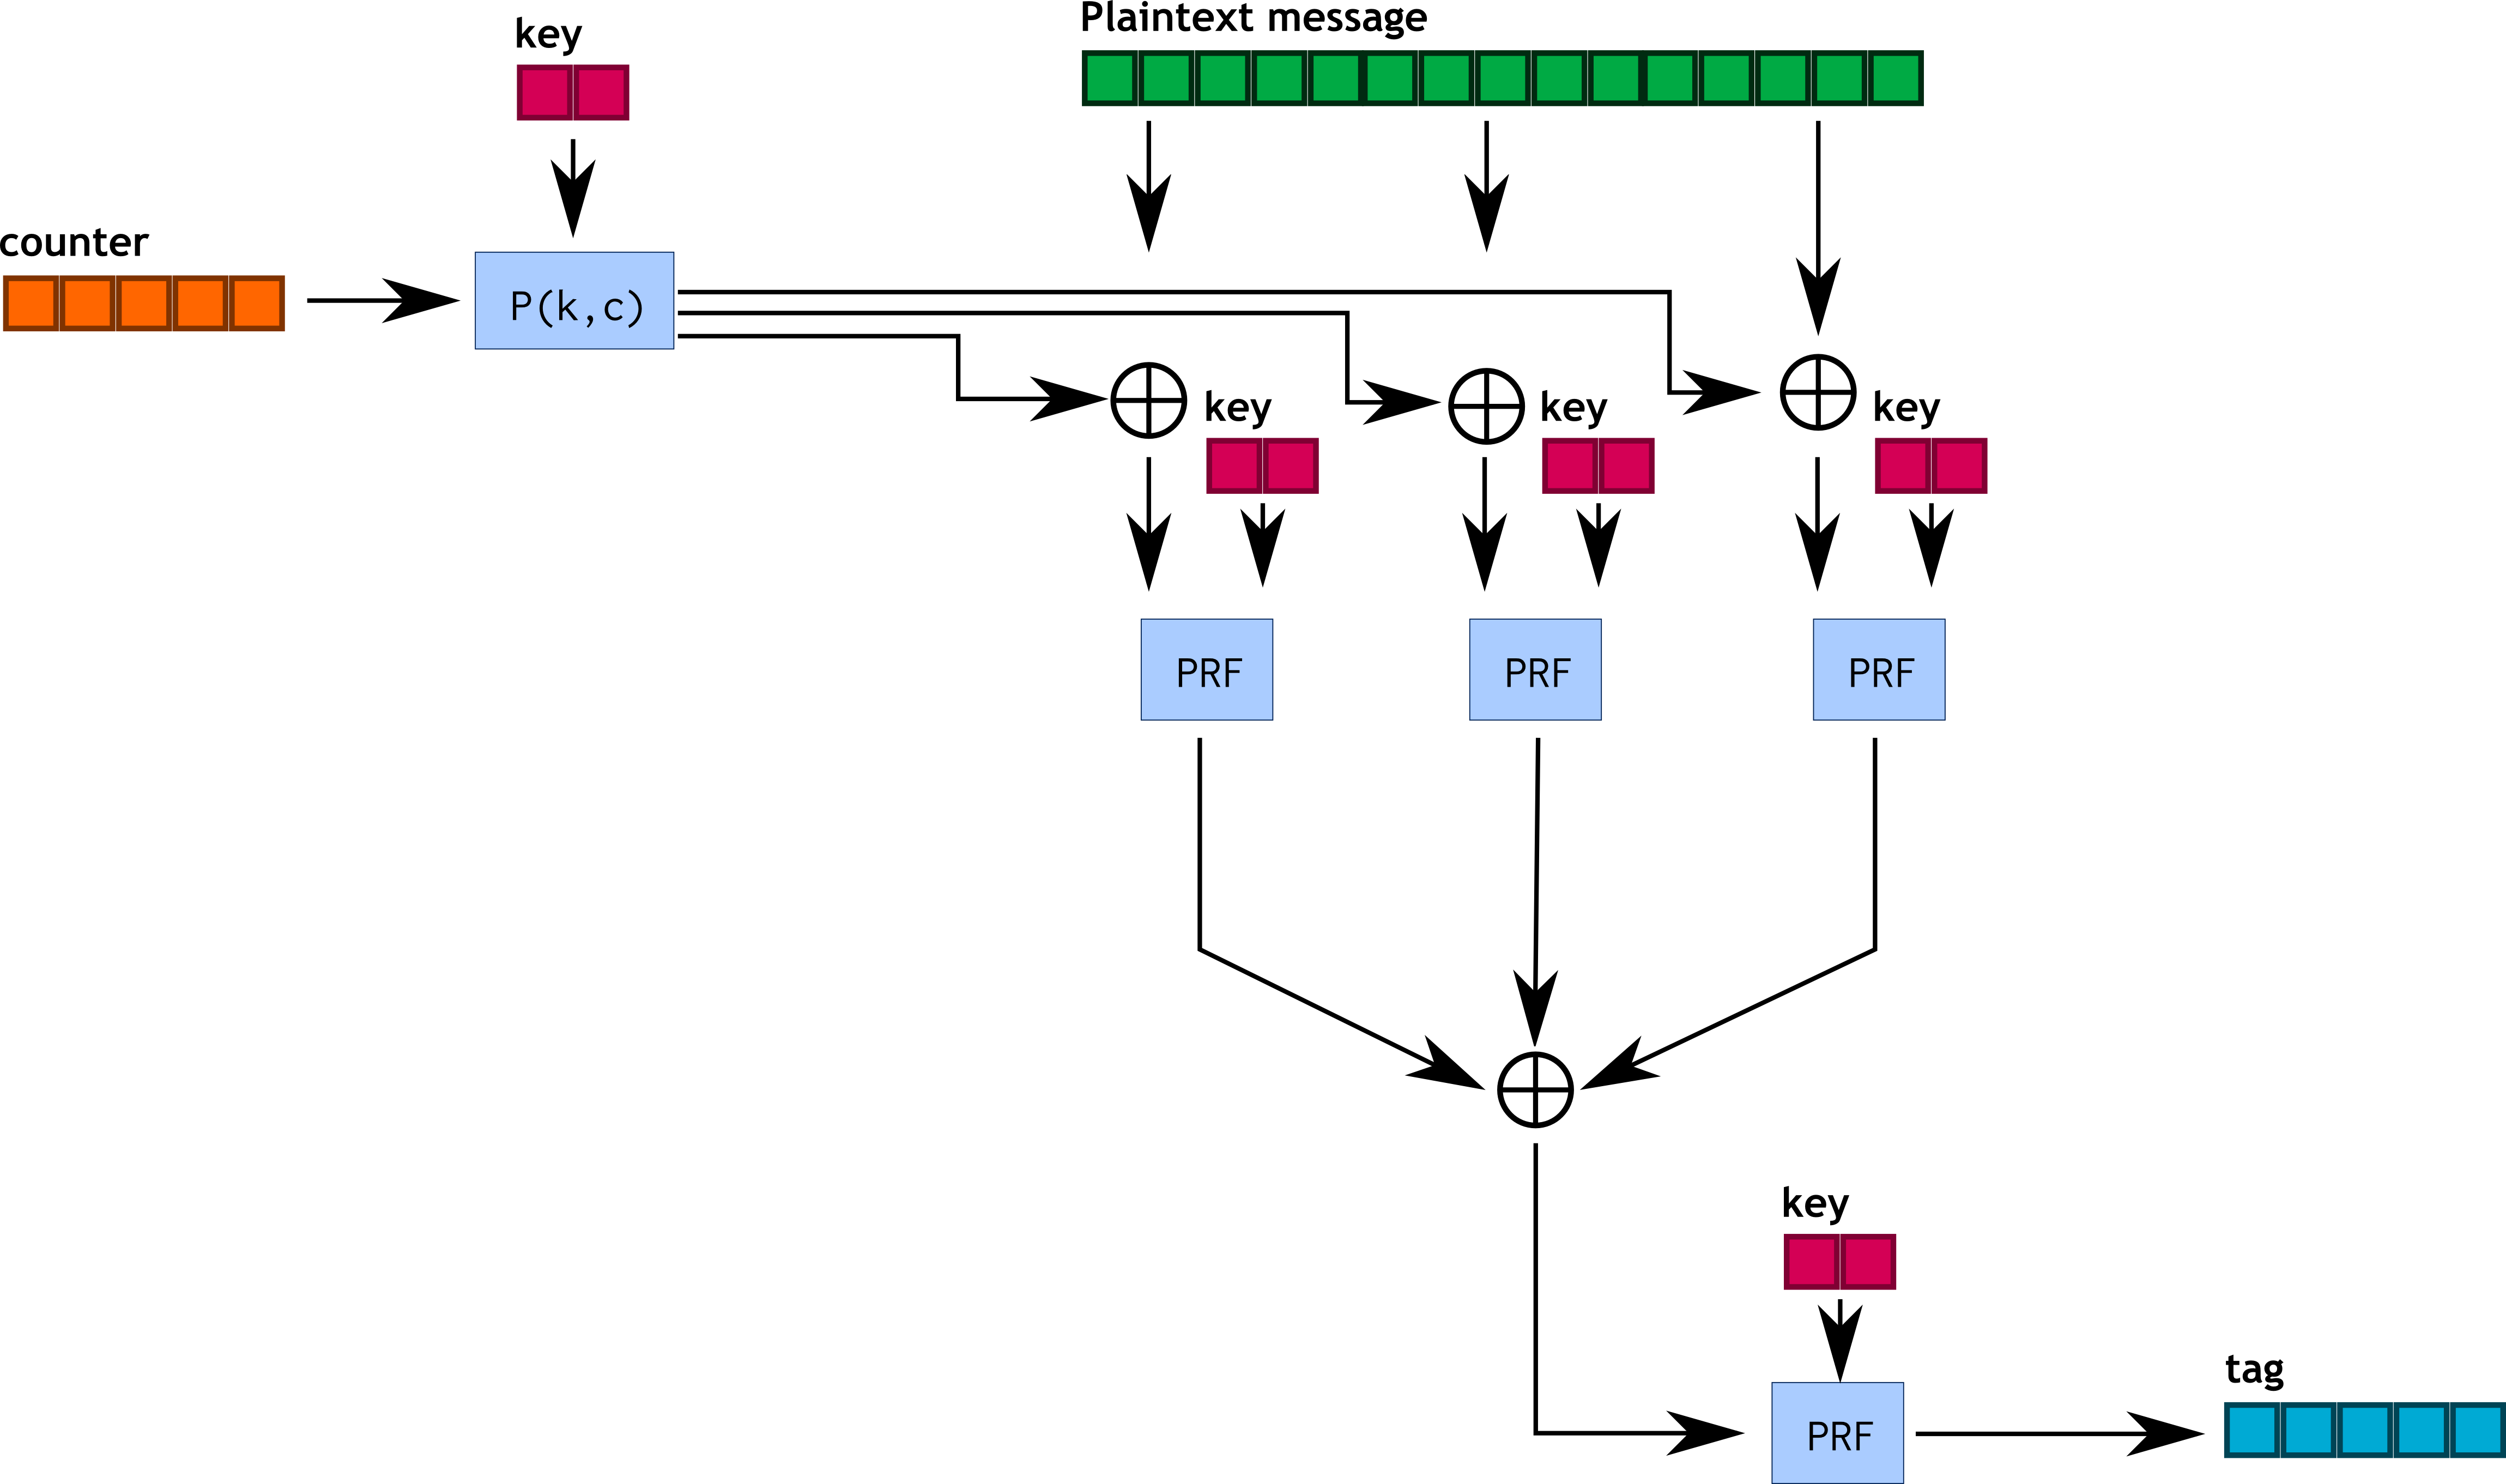
\includegraphics[width=0.7\textwidth]{PMAC.PNG}
	\caption{PMAC construction}
	\label{fig:PMACConstruction}
\end{figure}

The PMAC, or Parallel MAC, is obviously a parallel MAC construction : $P$ is a simple expansion function which will be used to fuzz the input data for each hash block. Like the previous constructions, the overall result is padded and hash one last time a second time to prevent oracle attack.

\begin{mytheorem}
	For every q-query adversary A attacking the PMAC, there exist an adversary B attacking the PRF function F such that : 
	\begin{flushright}
 		$Adv_{PRF}[A,F_{PMAC}] = Adv_{PRF}[B, F] + 2\times \frac{q^2\times L^2}{|X|}$	
	\end{flushright}
\end{mytheorem}



\subsection{Construction from hash functions}

There is another method to construct secure MAC, from collision-resistant hash functions. A lot of famous MAC use this construction : SHA-1, SHA-2, etc.

\paragraph{Compression functions}

Compression functions are function that map two domains (let call them $M$ and $T$) with the following property : the output domain $M$ is several orders of size smaller than the input domain $T$ ($|M| \ll |T|$). Compression functions often take a fixed-size message and a key and output a fixed-sized message, which halves the overall message length. \\
Collision resistance is a fundamental property for compression functions used in secure MAC mechanisms. Others useful properties : easily computable, pre-image and second pre-image resistance. \\
Compression functions are often constructed from ciphers : for example the Davies-Meyer construction use a encryption cipher and some fuzzying steps to produce a collision-based hash function. This construction has the advantage of saving space, since the cipher can be used to encrypt and hash data (more on \ref{sec:AuthenticatedEncryption}).

\paragraph{Merkle-Damgard Paradigm}

The Merkle-Damgard architecture is a general layout to construct secure MAC mechanisms from collision-resistant hashing functions. It relies heavily on compression functions :

\begin{figure}[h!]
	\centering
		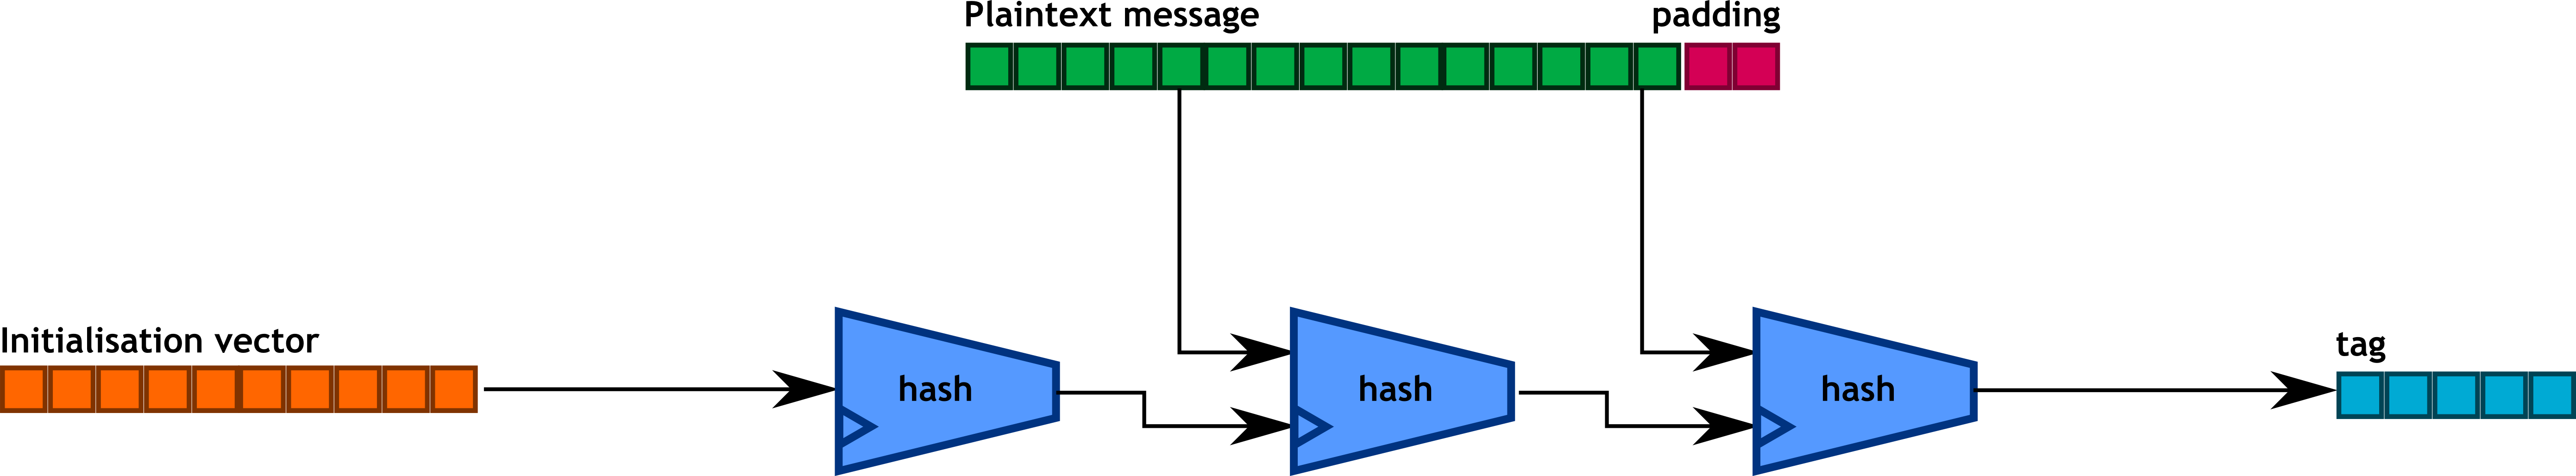
\includegraphics[width=0.7\textwidth]{Merkle-Damgard.PNG}
	\caption{Merkle-Damgard construction}
	\label{fig:MerkleDamgardConstruction}
\end{figure}

The construction is really similar to block ciphers : there is an initialization vector $IV$ to prevent replay attacks, several chained blocks of the same compression function, and a final padding. 

\paragraph{HMAC}

HMAC has two padding system : the inner pad $ipad$ and the outer pad $opad$.

\begin{figure}[h!]
	\centering
		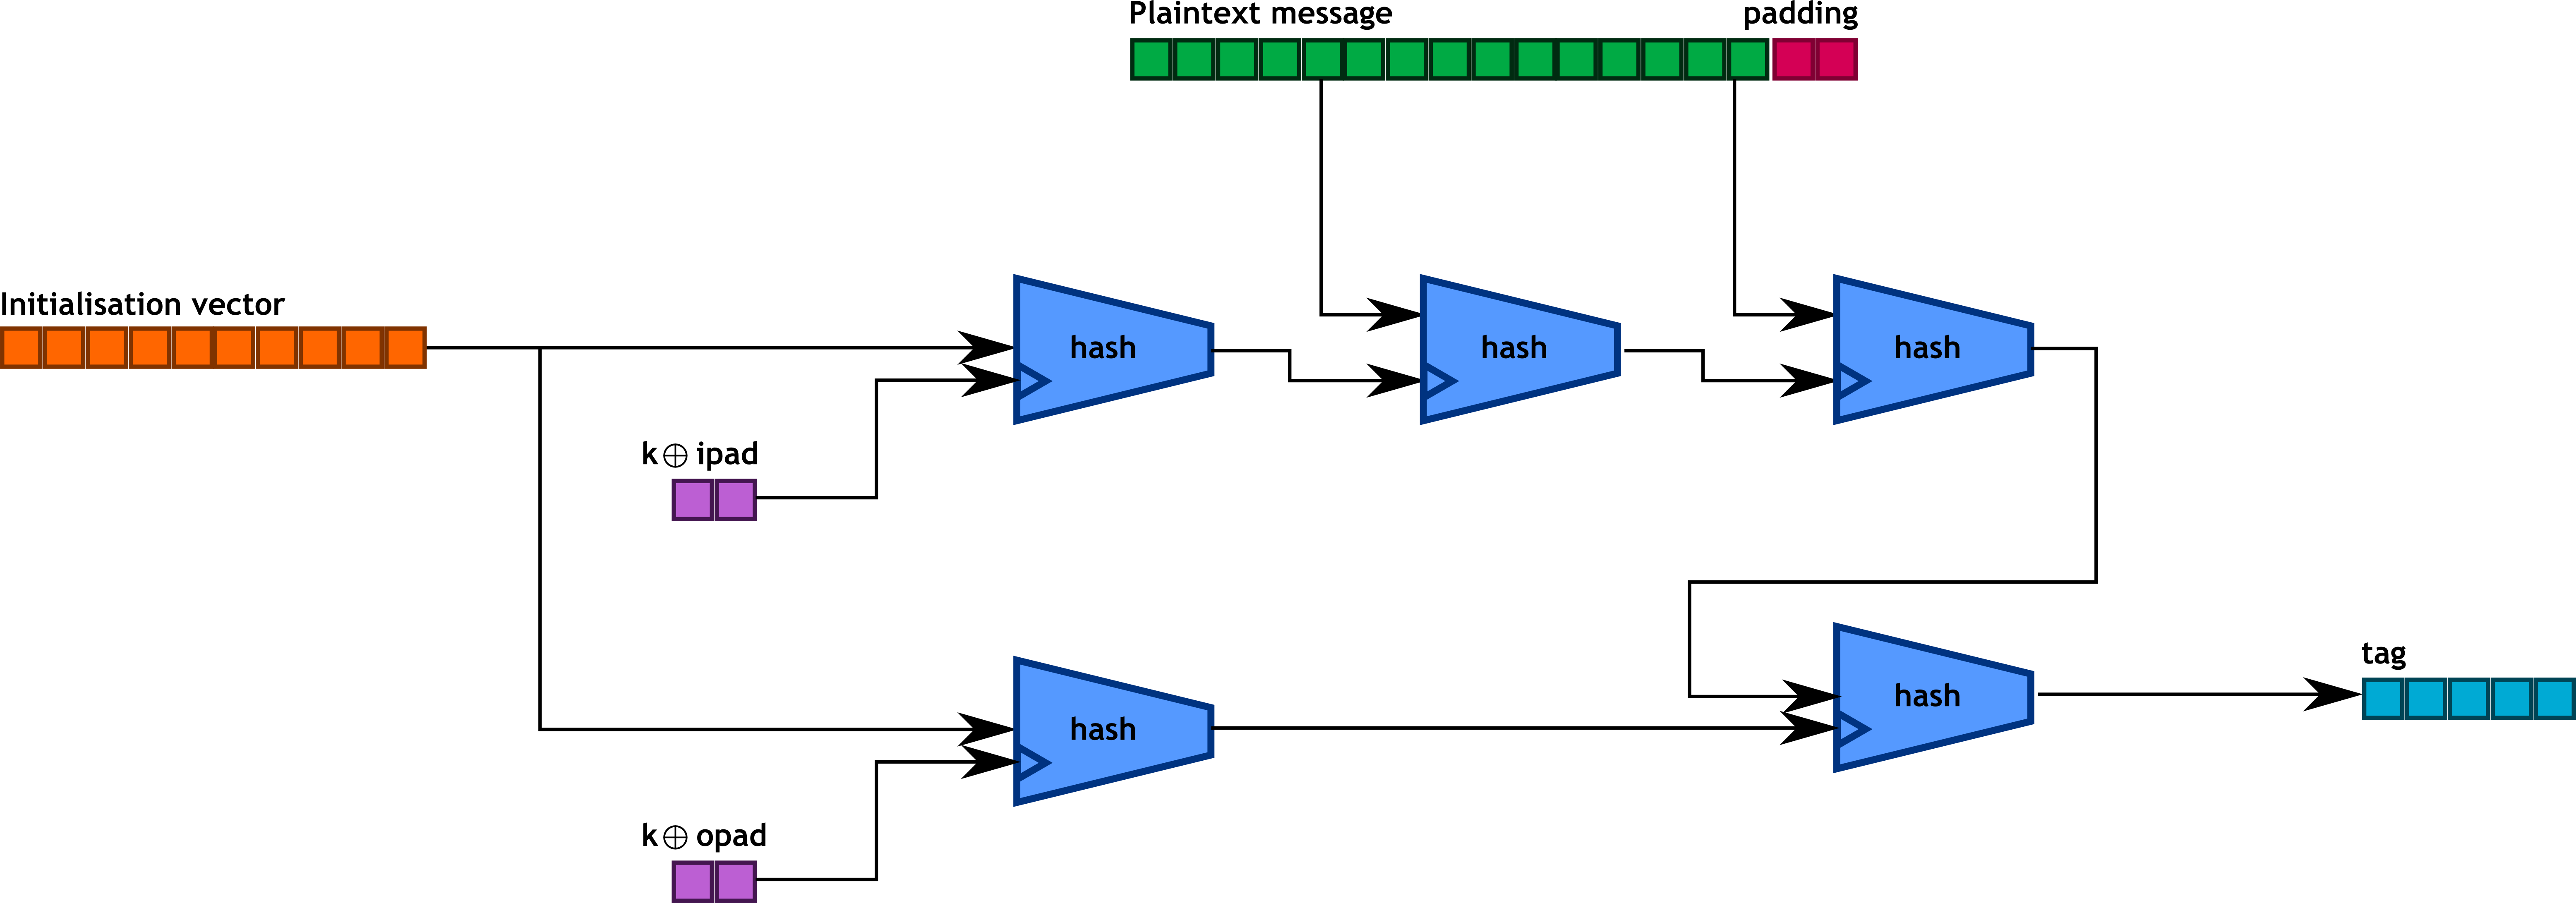
\includegraphics[width=0.7\textwidth]{HMAC.PNG}
	\caption{HMAC construction}
	\label{fig:HMACConstruction}
\end{figure}

\section{Authenticated Encryption}	
\label{sec:AuthenticatedEncryption}

Authenticated encryption is the following step in cryptography : ensuring integrity as well as confidentiality. In order to do that, it has to mix a MAC mechanism and a encrypting cipher. There is three approaches to the mixing :

\begin{description}
	\item[Encrypt-then-MAC :] This is the standard method, which yield the best results in terms of security.
	\item[Encrypt-and-MAC :]  Used for SSH.
	\item[MAC-then-Encrypt :] Used for SSL/TLS.
\end{description}


\subsection{Definition}

An authenticated encryption system consist of a cipher $(E,D)$ where : 
\begin{itemize}
	\item $E: KxM -> C$
	\item $D: KxC -> M\cup{\perp}$  ($\perp$ is the rejection symbol).
\end{itemize}

The system decrypt a ciphertext only if the MAC associated with has been validated. Otherwise, it will just output $\perp$. This symbol is important since it can prevent against oracle padding attacks : whether it's a invalid MAC or a pad error, the system has to output the same symbol in both cases.